
\chapter{Steuergerät}

Das Steuergerät, auch als Fahrrad-Bordcomputer bekannt, ist ein entscheidender Bestandteil eines E-Bike-Systems. Es dient dazu, die verschiedenen Betriebsmodi des Controllers zu steuern und dem Fahrer die Möglichkeit zu geben, die Einstellungen und Leistungsparameter des E-Bikes je nach Bedarf anzupassen.

\section{Umsetzung des Steuergeräts}

Die Umsetzung des Steuergeräts kann auf verschiedene Arten erfolgen. Eine Möglichkeit besteht darin, einen einfachen Schalter zu verwenden, der dem Fahrer die Wahl zwischen verschiedenen Modi bietet. Dieser Schalter kann beispielsweise zwischen den Modi für unterschiedliche Geschwindigkeitsstufen oder Leistungsniveaus umschalten.

Eine andere Möglichkeit ist die Integration eines anpassbaren Displays, das dem Fahrer eine visuelle Schnittstelle zur Steuerung des E-Bikes bietet. Mit einem solchen Display kann der Fahrer nicht nur zwischen verschiedenen Modi wählen, sondern auch Informationen wie Geschwindigkeit, Batterieladung und Fahrstrecke anzeigen.

Die Wahl zwischen einem einfachen Schalter und einem anpassbaren Display hängt von den individuellen Anforderungen und Präferenzen des Fahrers ab. Während ein einfacher Schalter eine unkomplizierte Bedienung bietet, ermöglicht ein Display zusätzliche Informationen und Anpassungsoptionen.

\section{Gründe für ein Steuergerät}

Ein Fahrrad-Bordcomputer bietet eine Vielzahl von Gründen und Vorteilen, die das Fahrerlebnis bei E-Bikes verbessern können. Einer der wichtigsten Gründe ist die Kontrolle über die Beschleunigung. Mit einer Throttle kann der Fahrer das Drehgas langsam aufdrehen und so die Beschleunigung kontrollieren. Im Gegensatz dazu gibt ein Tretlager-Sensor nur an, ob gerade getreten wird, und der Motor gibt automatisch die volle Beschleunigung. Dies kann zu unerwünschten Situationen und Gefahren führen, insbesondere in anspruchsvollen Gelände oder beim Starten an Steigungen.

Ein weiterer relevanter Aspekt ist die Möglichkeit, Motorparameter über den Bordcomputer einzustellen. Viele E-Bikes bieten verschiedene Unterstützungsstufen, die bestimmen, wie viel zusätzliche Leistung der Elektromotor beim Treten bietet. Über den Bordcomputer kann der Fahrer die gewünschte Unterstützungsstufe auswählen, die seinen Vorlieben und den Anforderungen der Strecke entspricht. Darüber hinaus ermöglicht der Bordcomputer die Anpassung der maximalen Geschwindigkeit des Motors, was besonders nützlich ist, um die Konformität mit lokalen Vorschriften einzuhalten oder persönliche Präferenzen zu berücksichtigen. Die Einstellung des Startverhaltens beeinflusst, wie schnell der Motor reagiert, wenn der Fahrer mit dem Treten beginnt, und einige E-Bikes bieten die Möglichkeit, zwischen verschiedenen Startmodi zu wählen, um den Fahrkomfort und die Sicherheit zu verbessern.

Des Weiteren kann der Bordcomputer den Rekuperationsmodus steuern, der bestimmt, wie stark der Motor beim Bremsen oder Bergabfahren Energie zurückgewinnt. Dies trägt nicht nur zur Effizienz des E-Bikes bei, sondern auch zur Erhöhung der Reichweite.

Zusammenfassend bietet ein Fahrrad-Bordcomputer zahlreiche Funktionen, die das Fahrerlebnis bei E-Bikes verbessern können. Von der Kontrolle über die Beschleunigung bis zur Anpassung von Motorparametern bietet der Bordcomputer eine Vielzahl von Möglichkeiten, um die Fahrt sicherer, komfortabler und individueller zu gestalten.

\section{Wahl des Steuergeräts}

Es ist nicht unbedingt erforderlich, ein Steuergerät zu verwenden, da die meisten Controller es ermöglichen, den Motor mit einer Throttle oder einem Tretlager-Sensor zu starten. Jedoch bietet ein Steuergerät eine bessere Kontrolle über das Fahrzeug. Bei der Verwendung einer Throttle kann der Fahrer das Drehgas langsam aufdrehen und so die Beschleunigung kontrollieren, während ein Tretlager-Sensor automatisch die volle Beschleunigung gibt, sobald mit dem Treten begonnen wird, was zu Gefahren führen kann.

Ein Fahrrad-Bordcomputer kann auch verwendet werden, um Motorparameter festzulegen, wie zum Beispiel verschiedene Unterstützungsstufen, maximale Geschwindigkeit, Startverhalten, Rekuperationsmodus und Motorleistung. Die Wahl des Steuergeräts hängt von den individuellen Anforderungen und Präferenzen des Fahrers ab.

\begin{figure}[h]
    \centering
    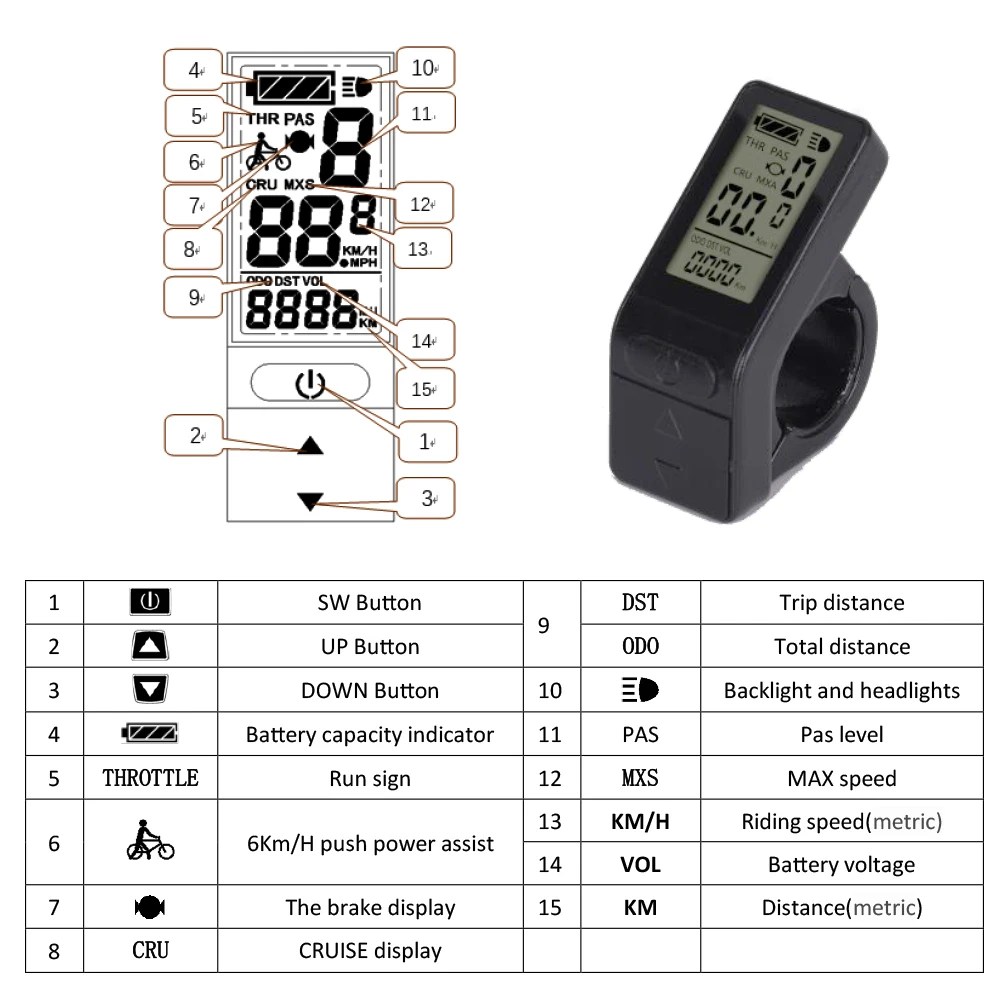
\includegraphics[width=8cm]{images/Elektrische-Bike-Display-KT-LCD4.png}
    \caption{KT LCD4\cite{noauthor_2822_nodate}}%
    \label{fig:14}
\end{figure}

In der Domäne der E-Bike-Technologie stehen verschiedene Steuergeräte zur Verfügung, die in ihren Funktionen und Einstellungen ähnlich sind. Dennoch variieren sie hauptsächlich im Bereich des Displays, des Designs und der Benutzeroberfläche, wobei die meisten über eine Standardausstattung von drei Bedienelementen verfügen, wie in Abbildung \ref{fig:14} dargestellt.

Die Wahl fiel auf das KT LCD4 Display aufgrund mehrerer Kriterien. Zum einen zeichnet sich das KT LCD4 durch seine minimalistische und kompakte Bauweise aus. Ein weiterer entscheidender Faktor war die Kompatibilität des KT LCD4 Displays mit dem vorhandenen Controller.

m Vergleich zu anderen Displays, die potenziell größer und sperriger sind, präsentiert sich das KT LCD4 als eine simple Lösung. Das minimalistisches Design und die benutzerfreundliche Oberfläche die sich nicht zu anderen unterscheidet machen es zu einer optimalen Wahl für das E-Bike-Projekt.

Im Anhang ist eine Abbildung eines alternativen Displays zu finden\ref{fig:15}, das zur Verfügung stand. Dieses zeichnet sich durch seine größeren Dimensionen und klobigeres Erscheinungsbild aus, was nicht mit dem Platzangebot des Lenkers kompatibel war. Das größte Problem ist jedoch, dass es nicht mit dem neuen Controller kompatibel ist.



%Zwei steuergerät welche funktionen haben sie?

%KT LCD4

\section{Konfiguration des Steuergeräts}





